\section{Introduction}
For digitization projects, the construction industry is yet a mostly unconquered field.
Complex dynamics and sometimes harsh (e.g. weather influence, no infrastructure, etc.) environments of construction sites challenge the technology and adds harder requirements compared to an industrial application on a shop floor. 
Moreover, the typically conservative and hierarchical work culture makes the introduction and acceptance of new methods more challenging. In this paper, we describe the vision and ideas behind the ConWearDi project and its approach to better understand and overcome these challenges.

\section{Project scope}
Construction projects vary highly in size and complexity from huge civil engineering projects to building a small house. 
The ConWearDi project focuses its efforts on improving efficiency of smaller constructions, e.g. interior work, painting of houses, and craftsman businesses.
Challenges included for such business are different than those a big multinational corporation with thousands of workers has to face, but nonetheless very interesting and important.

\section{Problem description}
The construction industry shows huge potential for digitization and is still in the early phase of adopting technologies related to Industry 4.0. 
While Building Information Modeling (BIM) is used more frequently for processes of the design and planning phase, the actual construction and execution process of the value creation, is still dominated by analog processes and paper documents. 
Examples include wall sized printed plans and time sheets on paper, which are adjusted with delay and only digitally recorded in offices, only available there. 
So, in many cases, the digital world ends in the back office or at the workstations of the architects, managers and foremen. 
The potential of novel services, such as Internet of Things (IoT) systems with sensors and actuators deployed on site connecting it to powerful computing resources, remained untapped.

\section{Project goal}
The goal of the ConWearDi project is the design and prototype implementation of a platform capable to capture and analyze the current state of construction work and to provide useful informational support not only for the managers and architects but directly to the construction workers and craftsmen on site. 

%Information sources, which provide structured information and accurate specifications (e.g. used materials) about a project, such as the BIM itself, are the foundation to achieve this goal. These

The main project goals can be summarized as:
\begin{enumerate}
  \item Creation of a Digital Twin, a representation of the construction site, which always reflects its current state 
  \item Centralized system for managing the construction site
  \item Automatic documentation for knowledge- and quality management purposes
  \item Exploration of new business models
  \item Development of methods for monitoring the activities of different worker groups with wearable technologies
\end{enumerate}

\section{Vision}

\begin{figure*}[htp]
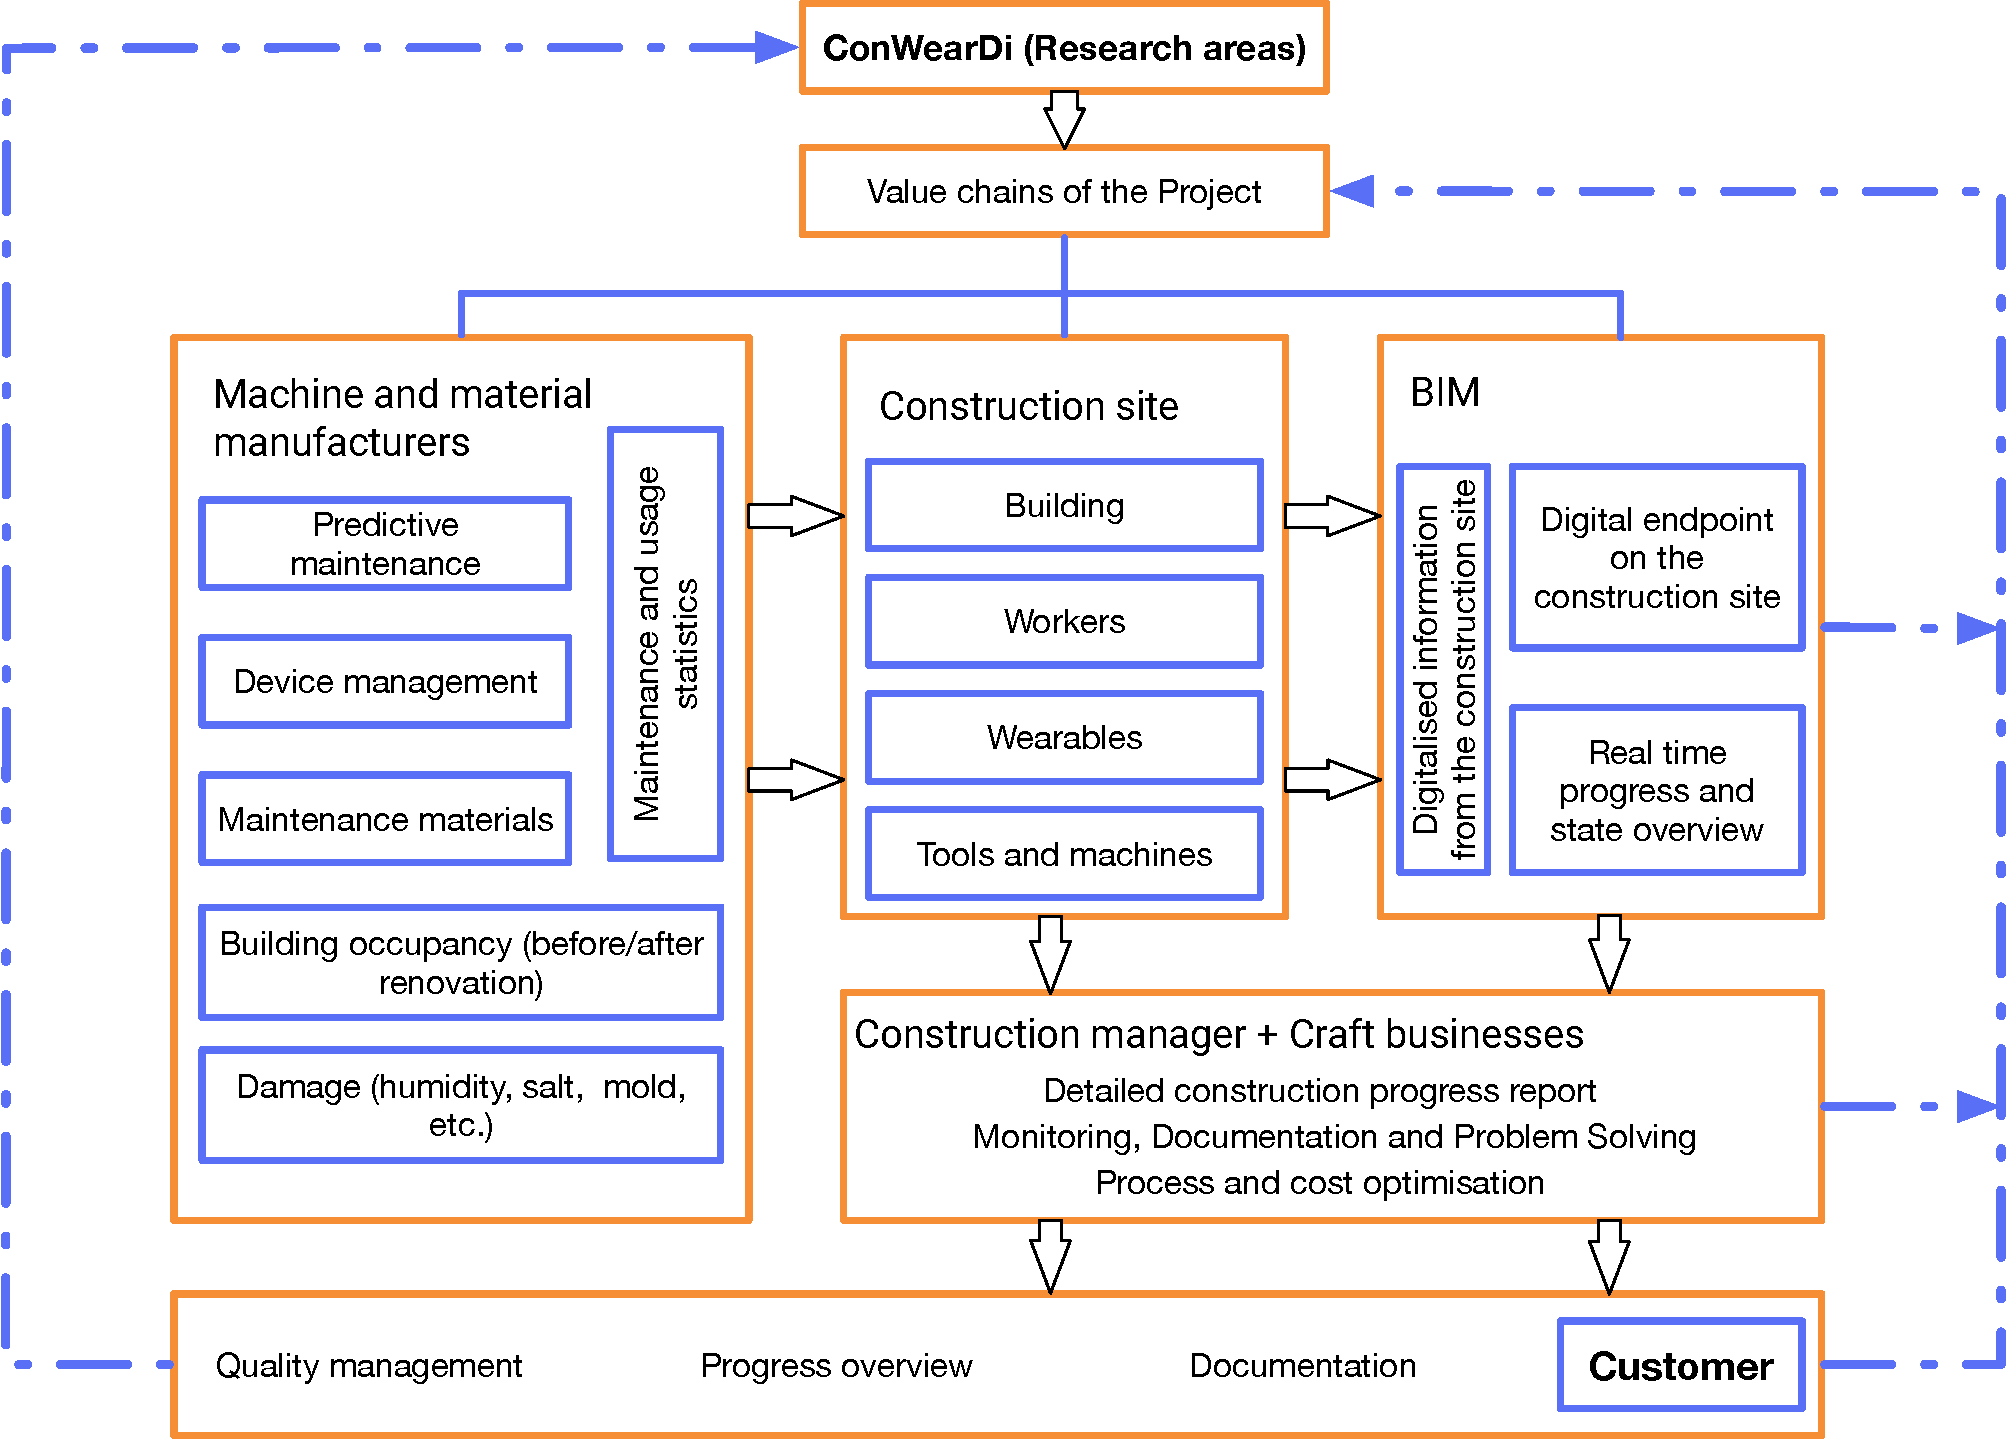
\includegraphics[width=0.8\textwidth]{figures/conweardi-functional.pdf}
\caption{Functional graph}
\label{fig:functional}
\end{figure*}

The most significant benefit, we envision through realization of the ConWearDi system, is better efficiency in detecting and preventing problems and damages by improving or if possible fully automatizing construction site documentation and reporting workflows.
With the real time information flow from the construction site, planners and managers are able to anticipate upcoming issues and avoid costly delays and damage repairs.
Communication between customers, managers, designers and workers will also be improved by bundling of information such as agreements, used materials, tools and recorded working hours. 

All in all, every stakeholder in the construction process will benefit from such a system.
In the following paragraphs, we describe what new or improved services each participant of the process would be able to use during the execution of their role.


\subsection{Construction site manager}
Similar to industrial control processes, the construction site's current state would be available real time through its digital twin.
This could help to recognize and avoid execution problems, e.g. when storage levels of the required materials running low.
The auto-generated reports unload this time consuming task from the construction manager, and allow also a more detailed documentation over time, saving the full history of the building creation.
This has major impact in later phases of construction or even in an other phases of the building's life cycle, when previous decisions can be retraced and interface problems can be recognized. 

Through the constant monitoring, the construction manager has a powerful tool to fulfill his responsibilities about work safety and protecting the employees health. In a simple example, this can mean to prevent health risk caused by overtime or using heavy machinery longer than allowed.
The accumulated knowledge can be used in other projects by learning from previous experiences (e.g. objective analysis of what went well, what went wrong).

\subsection{Designer and project coordinator}
The coordination process can rely on digitally documented commitments instead of verbal agreements, since they are just as simple to create.
The project coordinator also benefits from the simplified, IT-supported trade-coordination based on the methods of Advanced Planning and Scheduling (APS).
The process of automatic documentation can be easily adapted later to support new standards and regulations, e.g. for fire safety.
The high resolution data can be fed into big data analytics services, e.g. to detect patterns across multiple construction projects.
This allows new possibilities to improve organizational processes.

\subsection{Machine and tool manufacturers, material suppliers}
For machine, tool and material producers and suppliers, the increased connectivity of their devices and their integration into the digital processes of their customers helps to better understand the market and customer behaviors. 
Based on the collected information, they can implement more efficient service and logistic coordination e.g. by predicting when will be the customer's material storage depleted.

They can offer a proactive maintenance service for construction site machines based on their usage and wear tracking. 
Furthermore, machine manufactures can adapt new business models which rely on the connectivity and the sensors of their machines. An example is the just in time machine leasing, where customers pay only for the time when they really used the machine.


- Proaktive Instandhaltung von eingebauten Materialien durch Tracking von Zustand und bauphysikalischen Daten (z.B. Feuchte, Temperatur) 
- Fortwährende Erkenntnisse über Verbesserungs- und Optimierungspotenzial auf der Grundlage kontinuierlicher Sensordaten


\subsection{Craftsman businesses and construction workers}
- kontextbezogene, rückfragefreie Informationen zur Sicherung der Ausführungsqualität und Arbeitssicherheit
- Echtzeit-Remote-Supportmöglichkeiten zu allen Beteiligten (Planer, Maschinen- und Materialhersteller, Unternehmer)
- Meldewesen für Störungen und Integration jedes Einzelnen in den kontinuierlichen Verbesserungsprozess, dadurch Erhöhung der Arbeitszufriedenheit
- Echtzeit-Produktivitätsmessung, Soll-/Ist-Abgleich prozessorientierter Arbeitsablaufpakete mit der Möglichkeit zur Simulation von Alternativen
- optimierter Ressourceneinsatz und Entscheidungsunterstützung durch intelligentes, variantenfähiges Scheduling anhand von digitalen Echtzeitdaten von der Baustelle


\section{Methodology}
\todo{to succeed with the complex task - include experts from different professions and stakeholders}
\todo{figure describes the main functional process of the project - ... describe here }
Figure \ref{fig:functional}

\todo{project partners, who is doing what}

\todo{add paper references here to previous works of the groups}

Die Prozessverschiebung digitaler Endpunkte erfolgt in die wertschöpfenden Tätigkeiten auf der Baustelle, der eigentlichen Bautätigkeit. Zu diesem Zweck werden im Projekt ein Baugerätehersteller (Firma Wagner, Spritzmaschinen), ein Materialhersteller (DAW), ein mittelständischer Hersteller von ERP Software für Bauunternehmen (Sander + Partner GmbH), mehrere Handwerks-/Baubetriebe sowie Forschungsgruppen aus den Bereichen Internet of Things (DFKI), Prozessplanung (ITWM + eBZ) und Psychologie (TU KL) zusammenarbeiten. Seitens der Technologie werden die Baumitarbeiter mit Wearables (tragbare Computersysteme) ausgestattet und auf der Baustelle kommen intelligente Maschinen (konkret z.B. Spritzmaschinen für Malerarbeiten), sowie in Materialien integrierte Sensoren zum Einsatz (z.B. Sensoren in der Wärmedämmung).

Dabei sollen Lösungen erarbeitet werden die es (1.) Geräteherstellern erlauben eine proaktive Wartung der Geräte auf der Baustelle vorzunehmen, (2.) Materialherstellern eine proaktive Instandhaltung der verbauten Materialien, (3.) neue Geschäftsmodelle ermöglicht (z.B. “just in time”-Geräteleasing, kundenbezogen Marketingmethode), und (4.) eine datengetriebene Weiterentwicklung der Produkte und Dienstleistungen durch von vielen Kunden gesammelte „BigData“ erlauben. Des Weiteren sollen reale Bauprozesse durch digitale Echtzeitinformation ihrer Repräsentation in den ERP-Systemen synchronisiert werden. So können Bauprozesse im Sinne von Effizienz, Qualitätssicherung und Arbeitssicherheit überwacht und gesteuert werden. Dadurch kann auch dem Baukunden ein einmaliger vertrauensbildender Zugang und eine einmalige Dokumentation zum Bauprozess als Dienstleistung geboten werden.
Die aufgeführten Projektergebnisse sind in der nachfolgenden Funktionsgrafik in ihrer Wirkungsbeziehung dargestellt.


\section{Conclusion}
\todo{high potential to digization - still many unsolved problems - project is focusing to making first demonstrators - running at first real businesses}

\todo{for more information visit project website}

\begin{acks}
  This work has been funded by the Federal Ministry of Education and Research of Germany (BMBF) within the framework of the project ConWearDi.
\end{acks}
